%&pdflatex
\subsection{Partizioni per Debian}
Dobbiamo a questo punto selezionare lo spazio libero sul disco, come in Figura \vref{fig:select-free-space}.

\begin{figure}[ht]
	\centering
	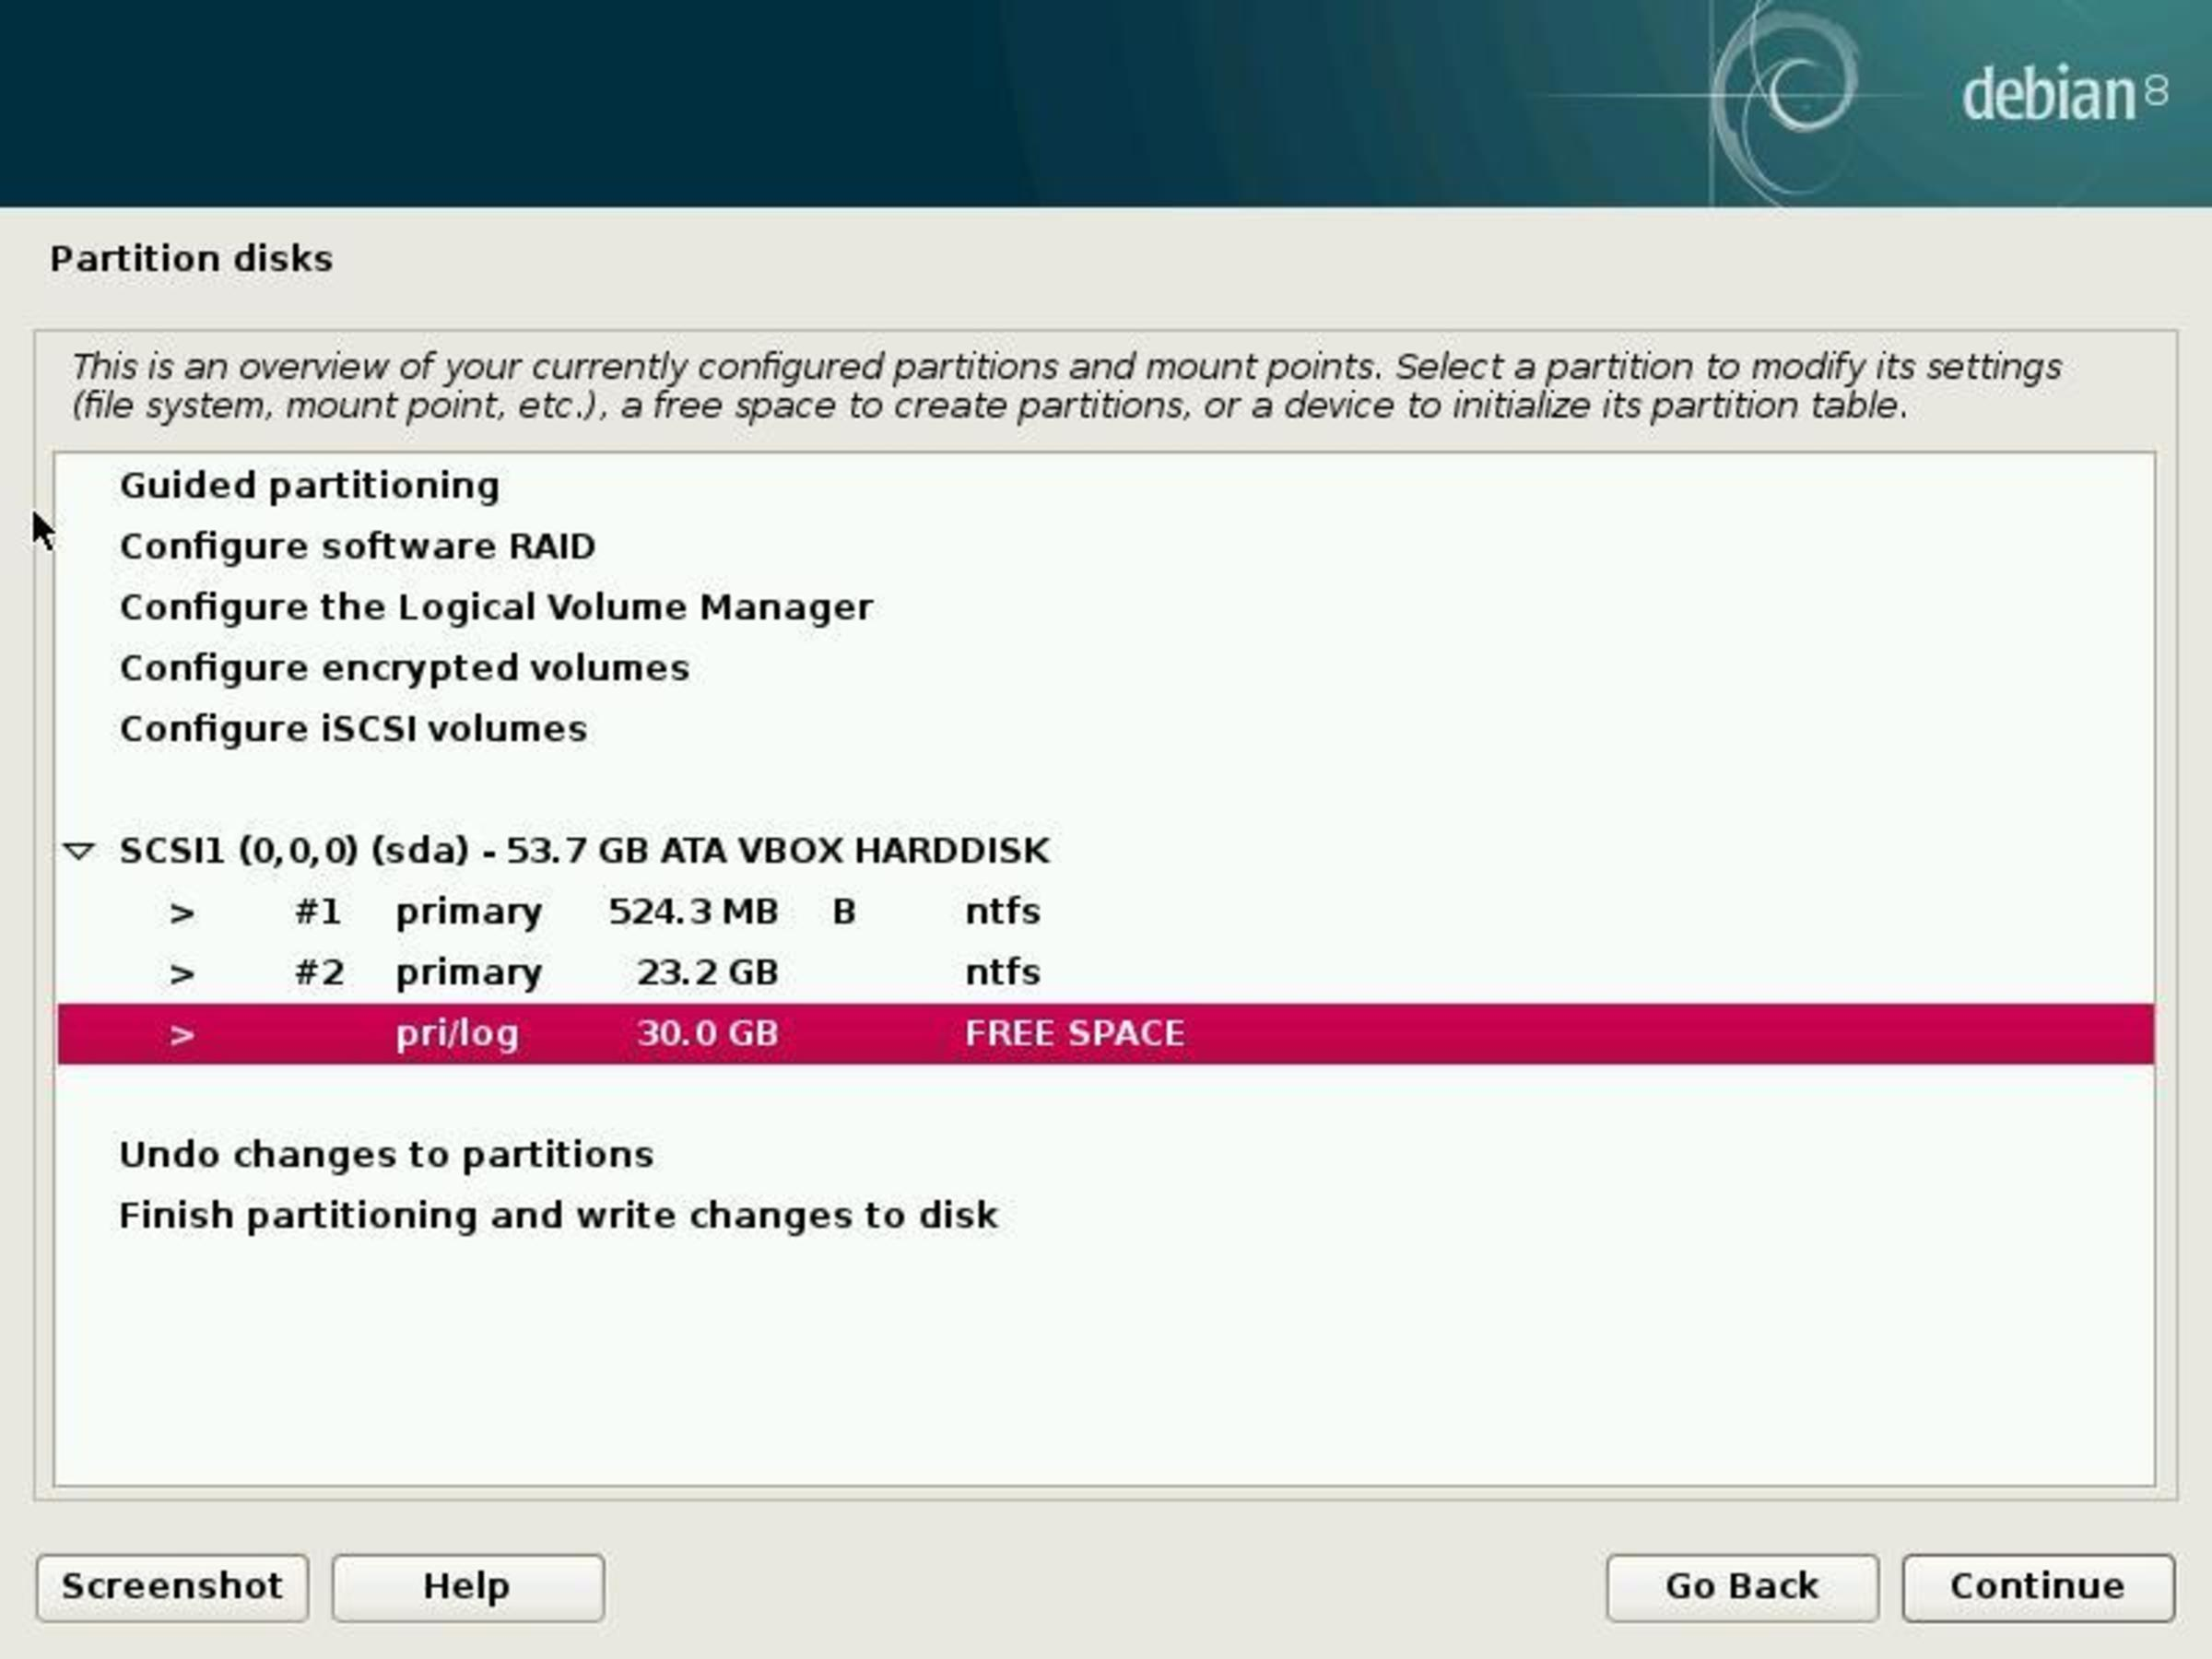
\includegraphics{select-free-space}
	\caption{Selezione dello spazio libero da utilizzare per le partizioni di Debian}
	\label{fig:select-free-space}
\end{figure}

Nella schermata successiva, selezioniamo \texttt{Automatically parti\-tion the free space} (\texttt{Partizionare automaticamente lo spa\-zio libero}). A questo punto saremo ricondotti al partizionamento guidato di Figura \vref{fig:partitioning}. Si scelga il partizionamento preferito (consigliamo di evitare di separare \texttt{/var} e \texttt{/tmp}).

\begin{figure}[ht]
	\centering
	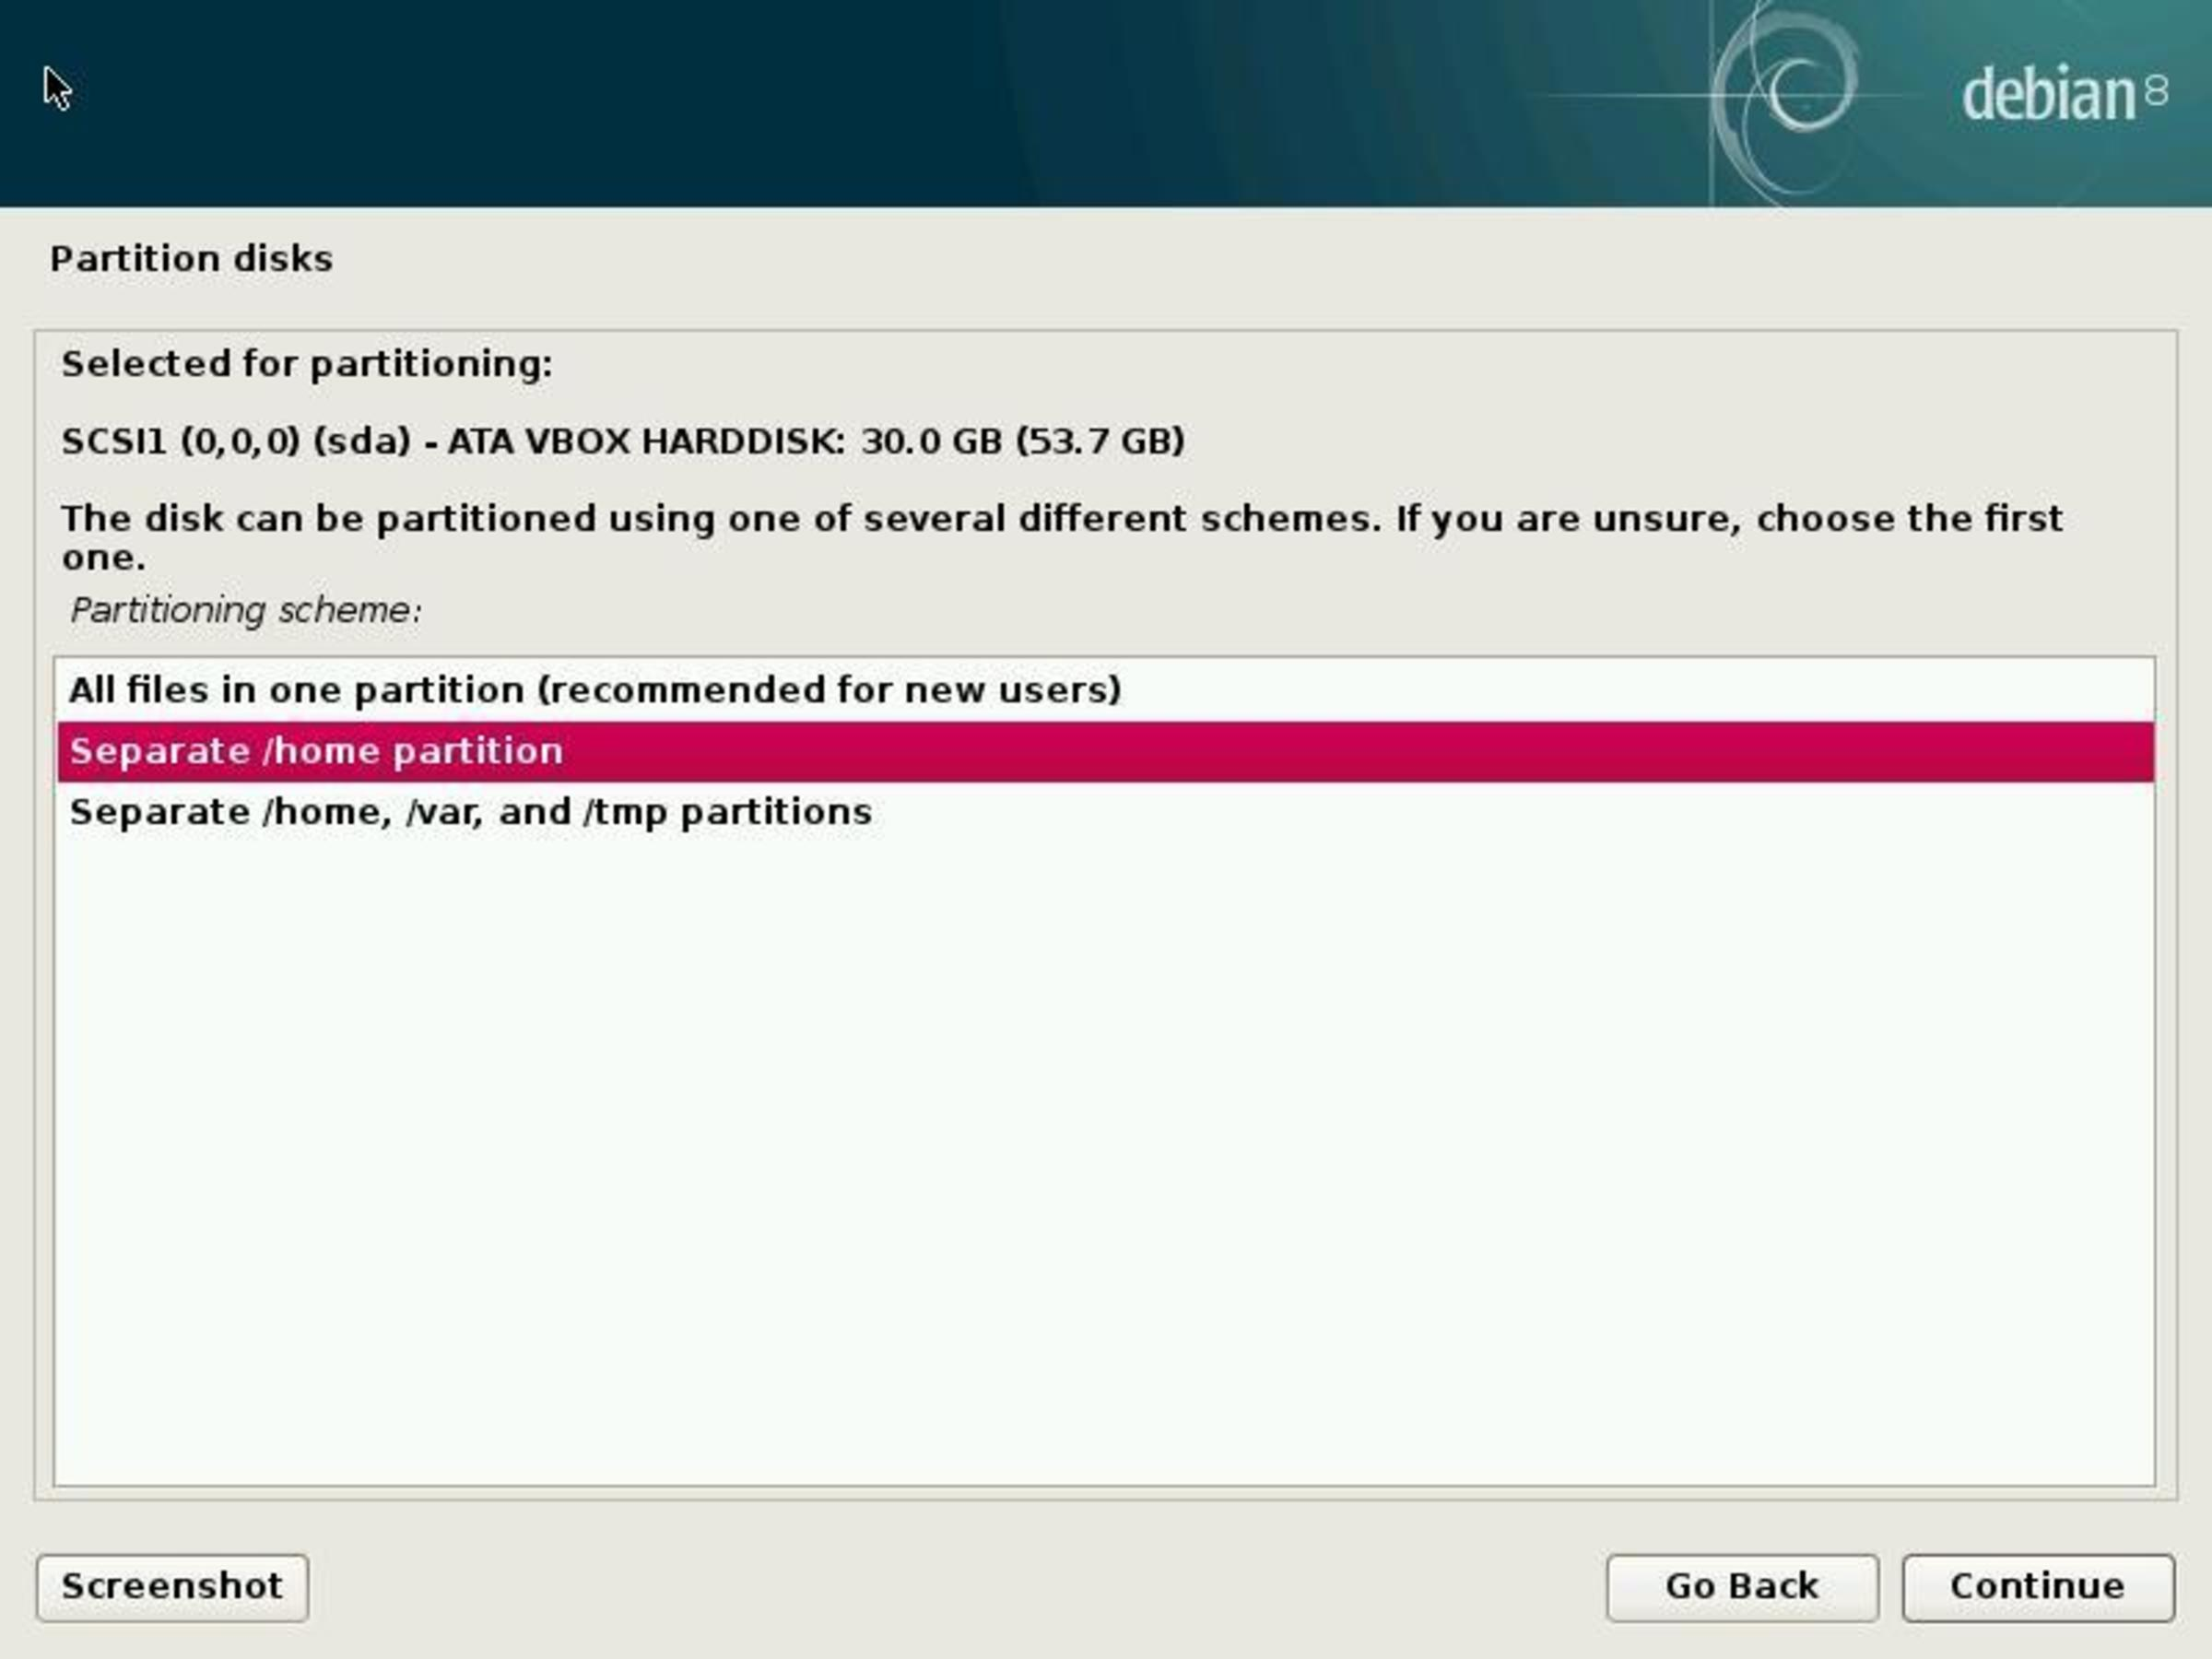
\includegraphics{partitioning}
	\caption{Selezione dello schema delle partizioni con partizionamento guidato}
	\label{fig:partitioning}
\end{figure}

A questo punto Debian ci farà vedere lo schema finale. Selezioniamo quindi \texttt{Finish partitioning and write changes to disk} (\texttt{Terminare il partizionamento e scrivere le modifiche sul disco}). Rispondiamo affermativamente alla domanda di conferma di scrittura delle modifiche su disco. Debian a questo punto salverà le nuove partizioni e inizierà ad installare il sistema di base.
